%%
%% This is file `sample-sigconf.tex',
%% generated with the docstrip utility.
%%
%% The original source files were:
%%
%% samples.dtx  (with options: `sigconf')
%% 
%% IMPORTANT NOTICE:
%% 
%% For the copyright see the source file.
%% 
%% Any modified versions of this file must be renamed
%% with new filenames distinct from sample-sigconf.tex.
%% 
%% For distribution of the original source see the terms
%% for copying and modification in the file samples.dtx.
%% 
%% This generated file may be distributed as long as the
%% original source files, as listed above, are part of the
%% same distribution. (The sources need not necessarily be
%% in the same archive or directory.)
%%
%% The first command in your LaTeX source must be the \documentclass command.
\documentclass[sigplan,screen]{acmart}

\usepackage{code}
\usepackage{graphicx}
\usepackage{placeins}
\usepackage{tikz}
\usetikzlibrary{shapes, arrows, positioning}

%%
%% \BibTeX command to typeset BibTeX logo in the docs
\AtBeginDocument{%
  \providecommand\BibTeX{{%
    \normalfont B\kern-0.5em{\scshape i\kern-0.25em b}\kern-0.8em\TeX}}}

%% Rights management information.  This information is sent to you
%% when you complete the rights form.  These commands have SAMPLE
%% values in them; it is your responsibility as an author to replace
%% the commands and values with those provided to you when you
%% complete the rights form.


%%
%% Submission ID.
%% Use this when submitting an article to a sponsored event. You'll
%% receive a unique submission ID from the organizers
%% of the event, and this ID should be used as the parameter to this command.
%%\acmSubmissionID{123-A56-BU3}

%%
%% The majority of ACM publications use numbered citations and
%% references.  The command \citestyle{authoryear} switches to the
%% "author year" style.
%%
%% If you are preparing content for an event
%% sponsored by ACM SIGGRAPH, you must use the "author year" style of
%% citations and references.
%% Uncommenting
%% the next command will enable that style.
%%\citestyle{acmauthoryear}

%%% The following is specific to Onward! '24-ESSAYS and the paper
%%% '(Programs), Proofs and Refutations (and Tests and Mutants)'
%%% by Alex Groce.
%%%
\setcopyright{acmlicensed}
\acmDOI{10.1145/3689492.3689810}
\acmYear{2024}
\copyrightyear{2024}
\acmISBN{979-8-4007-1215-9/24/10}
\acmConference[Onward! '24]{Proceedings of the 2024 ACM SIGPLAN International Symposium on New Ideas, New Paradigms, and Reflections on Programming and Software}{October 23--25, 2024}{Pasadena, CA, USA}
\acmBooktitle{Proceedings of the 2024 ACM SIGPLAN International Symposium on New Ideas, New Paradigms, and Reflections on Programming and Software (Onward! '24), October 23--25, 2024, Pasadena, CA, USA}
\acmSubmissionID{onward24essays-p7-p}
%\received{2024-04-25}
%\received[accepted]{2024-08-08}

%%
%% end of the preamble, start of the body of the document source.
\begin{document}

%%
%% The "title" command has an optional parameter,
%% allowing the author to define a "short title" to be used in page headers.
\title{Mutation Driven Development}

\author{Alex Groce}
\orcid{0000-0003-0273-4668}
\affiliation{%
  \institution{Northern Arizona University}
  \city{Flagstaff}
  \country{USA}
}
\email{agroce@gmail.com}

%% By default, the full list of authors will be used in the page
%% headers. Often, this list is too long, and will overlap
%% other information printed in the page headers. This command allows
%% the author to define a more concise list
%% of authors' names for this purpose.
\renewcommand{\shortauthors}{Alex Groce}

%%
%% The abstract is a short summary of the work to be presented in the
%% article.
\begin{abstract}

\end{abstract}

\begin{CCSXML}
<ccs2012>
<concept>
<concept_id>10011007.10010940.10010992.10010998.10011001</concept_id>
<concept_desc>Software and its engineering~Dynamic analysis</concept_desc>
<concept_significance>500</concept_significance>
</concept>
<concept>
<concept_id>10011007.10011074.10011099.10011102.10011103</concept_id>
<concept_desc>Software and its engineering~Software testing and debugging</concept_desc>
<concept_significance>500</concept_significance>
</concept>
</ccs2012>
\end{CCSXML}

\ccsdesc[500]{Software and its engineering~Dynamic analysis}
\ccsdesc[500]{Software and its engineering~Software testing and debugging}

\keywords{test driven development, mutation analysis}



\begin{abstract}
Test driven development (TDD) is a controversial and interesting approach to
software development; while many think of ``better tests'' as a
primary \emph{purpose} of TDD, in practice the goal is as much to use
tests to encourage continued progress in coding.   That goal however
rests on the notion that TDD ensures tests are good enough to let you
implement small new features and refactor code without undue fear of
mistakes.  Unfortunately, TDD is not ``self-enforcing'' and standard
TDD practice makes it easy to accidentally skip steps.  By integrating
a phase of focused mutation testing into TDD, however, developers
applying TDD can be sure they are actually writing code that is
supported by the scaffolding of tests, and so code in justified confidence.  The incremental nature of TDD
test and production code creation ensures that at no point will
``fixing up'' the mutants be likely to overwhelm the developer, and so
the final result will be tests with excellent code coverage and
mutation score, without a painful effort to ``patch up'' an inadequate
testing effort, and a TDD approach that includes automated checks that
the letter and spirit of TDD are truly being respected, with the
benefits of TDD presumably following in due course.
  \end{abstract}



\maketitle


\section{Introduction}

The first question I should answer: given the abstract, which sounds
like a fairly standard software engineering research paper abstract,
except for the missing part bragging
about a positive experimental evaluation, why is this an Onward! Essay
and not a conventional research paper?

The answer is personal:  I thought of this idea a few years ago, and
have thought about making it a full research project off and on since
then, but I
never managed to actually do so.  A real evaluation of this idea would
require a good graduate student's devotion, and, more importantly,
actual human-subjects experimentation work to arrive at even a
speculative and provisional scientific evaluation of the idea's
efficacy.  I can't think of a useful way to make a purely ``extract
code from public repos and analyze it'' investigation, or (better yet)
a purely mechanical experiment.  Perhaps in a few years it will be
possible to just have LLMs do it all?

I (read: ``my lab'') don't really do human subjects; I don't ever want to
write IRB paperwork.  I do work with \emph{other people} who do human subjects,
from time to time; so I could potentially convince one of those
wonderful folks that this is a good project, and thus avoid doing IRB
paperwork and still make this a ``real'' paper.

But I don't have a huge committment to Test
Driven Development to get me excited enough to try to talk someone
else into spending valuable research productivity time on this idea; I've never used
TDD in writing code myself, and I'm not sure I even believe it's a good development
practice!  Nobody I know and trust in the real software industry seems
to do things in a TDD way, which is worrying.  So it just doesn't
seem worth it to commit to a serious Research Project, likely spanning
over a year, just to explore this idea (I have lots of other ideas
that I think are equally or more interesting, that I also don't have
time to make happen).

So why not do what we senior researchers usually do in this situation?
Shelve the idea, perhaps mention it to one or two people, and let it
basically die?  I've done this before; there are a good half-dozen
implmentations of test generation ideas I think might be interesting
or effective in my TSTL Python test generation tool~\cite{tstlsttt}, none of which
ever became a paper.  They live only as obscure command line options
to a tool increasingly few people are likely to ever use.  It's sad,
but life is short, and I don't think any of those ideas are likely to
be \emph{really} important, vs. somewhat, occasionally, useful.
Perhaps that's the right approach with Mutation Driven Development,
too.

Still, I didn't \emph{want} to do that; this idea has been bugging me
for years, and I have wondered if TDD is unappealing precisely for the
reasons that made me consider the idea of MDD, which are discussed
below.  Perhaps if TDD delivered more of what it promised, it would be
better, and more people I know would make use of it or some variation
of it?  I don't particularly ``believe'' in TDD (but I also don't hate
the idea; it has a certain formal elegance and logic), but I do
believe in mutation testing!  Furthermore, Dijkstra's ideas of proving small pieces of code correct are
also seldom if ever practiced, and certainly not by anyone I know in industry; should we
therefore throw them out?  Or work to make them practical and useful?
I wondered about these bigger-picture questions, and didn't throw the idea out of my head, even if I didn't
make any progress on it.

\subsection{Daniel Jackson Made Me Do It}

I recently read Daniel Jackson's \emph{The Essence of Software}~\cite{essence}, which
is a very enjoyable book.  The supposed topic of the book is an
approach to design that I thought was interesting, but that also seems
more appropriate to UI-heavy software than the
kind of code analysis/test generation software I tend to write
myself, or the kind of embedded or systems code (e.g. file systems and
compilers) I
tend to test.  The real value of the book was, for me, twofold:  first, the
long long set of ``notes'' after the main text is a delightful random
walk through software engineering.  Second, Jackson's musings include
a major theme:  we've become too careful in the software engineering
research community.  Given the heroic (for lazy computer scientists,
at least;
obviously many a research project in SE is not \emph{that} much work compared to
the work of serious systems people, much less biologists or
physicists) effort required for making Real Science that Has Six Good
RQs and Makes it Past the ICSE Program Committee, we tend to drop
marginal ideas, especially if we as researchers are not inclined to be
managers for an army of graduate students, but prefer instead to be
less-productive/more-hands-on (here's looking at myself in a mirror),
and have many fewer meetings and Slack conversations.

There was a time
when SE (or formal methods, where I was living at that time) was far
too accepting of a paper based on application of an approach to a
single toy problem, plus a good writeup.  This was too lacking in
rigor, and there was a very sensible effort to increase the level of
experimental support for claims about software engineering.  I don't
have a strong opinion on how this worked out for more methdological
aspects of SE, but for the most part the increased experimental
validation (and, later, statistical sophistication, or at least competence) was necessary to
make work in more ``technical'' parts of SE, such as software testing,
trustworthy.  In a minor way, I think I helped encourage this trend in
software testing, especialy under the influence of an unusually
statistics-savvy and very capable graduate student, Rahul Gopinath
(now faculty at the University of Sydney).

However, this increased rigor was not without a cost:  some of the most important and
influential papers in SE, as Jackson points out, did not rest on a
basis of experimental support, in part because they were more raw
``ideas'' than a narrower scientific claim.

Now, many researchers take ideas that don't satisfy the current rules
for \emph{proper} papers and turn them into blog posts or at least
tweets.  I've done this.  But there's an argument that this limits the
audience to people who already know who you are and watch what you
say.  If your ideas are relevant to another community, one you aren't
part of, this is likely to mean they never reach that audience.

In the past I've written Onward! Essays when the topic was clearly not
one suitable to a standard research paper.  This time, I'm writing an
essay because that seems more responsible than writing a blog post,
and a research paper minus the experimental evidence is just an
essay\footnote{This is a joke!  The related statement that an essay is
  just a research paper missing experimental evidence is, of course,
  even less true; an essay is a ``jackdaw, a magpie, a
  raven''~\cite{doyleessay}, and while some good research papers contain the germs of
  an essay, the two forms are generally distinct, not that you would
  be so sure of that from the example at hand, the essay you are reading.}.  The reader is free to try the idea out, with no guarantee that
it will work, but really --- we know that's the case with most
research, as well, except in the most unusual of circumstances.  So,
onward to the idea.



\section{What is Test Driven Development?}

\begin{figure}[h!]
  \centering
  \resizebox{\linewidth}{!}{%
    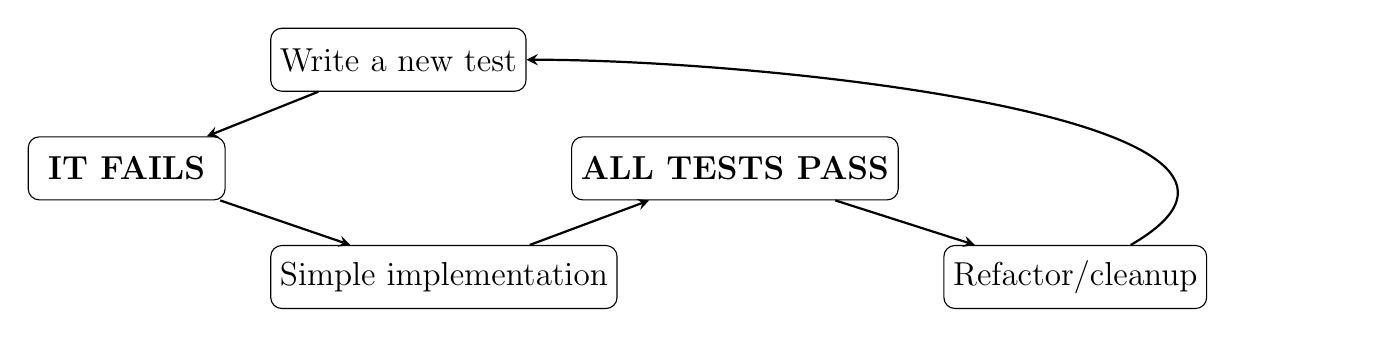
\begin{tikzpicture}[
      font=\large,
      node distance=0.8cm,
      box/.style={rectangle, draw, rounded corners, text centered, minimum width=2.5cm, minimum height=0.8cm},
      arrow/.style={thick,->,>=stealth}
    ]
      \node (write) [box] {Write a new test};
      \node (fail) [box, below left=of write] {{\bf IT FAILS}};
      \node (implement) [box, below right=of fail] {Simple implementation};
      \node (pass) [box, below right=of write] {{\bf ALL TESTS PASS}};
      \node (refactor) [box, below right=of pass] {Refactor/cleanup};

      \draw [arrow] (write) -- (fail);
      \draw [arrow] (fail) -- (implement);
      \draw [arrow] (implement) -- (pass);
      \draw [arrow] (pass) -- (refactor);
      \draw [arrow] (refactor) to[out=30,in=0] (write);
    \end{tikzpicture}%
  }
  \caption{Test-Driven Development Loop}
  \label{fig:tdd}
\end{figure}

Test Driven Development (henceforth TDD) has been defined many times~\cite{beck2002test,astels2003test,TDDIBM,TDDAcademy},
in many ways.  Even if you're familliar with TDD, I would like to
revisit the foundations for a moment, because the proposal made here
is formulated with respect to a particular conception of TDD.  Most
definitions of TDD (including this one) properly present it as a
\emph{series of steps to be followed in development}.

\begin{enumerate}
  \item Think of a behavior your software does not yet have,
    but that you want it to have.
    \item Add a test that would pass if that behavior was present, but
      will not pass if it is not.
    \item Run all your tests and see that the newly added test fails.
    \item Make a \emph{small} change that makes the test pass.
    \item Run all the tests; make sure they all succeed now.
      \item Refactor to remove duplication/generally clean the code
        from step 4 up so it doesn't make you ashamed of yourself.
        \item Repeat (go to 1).  Do not, generally, make changes other than by
          this process!
      \end{enumerate}

I added the first step, because you can't really write a test until
you've thought of something to test.  The basic process is as shown in Figure~\ref{fig:tdd}.


Why write software in this restrictive way?  The benefits proposed
vary, but I think can be summarized as:

\begin{itemize}
  \item By making such small steps, you always have the confidence to
    move forwards.  This may not be the first thing most people think
    of with TDD, but Beck's extremely influential book~\cite{beck2002test} really focuses
    on this.  You never get stuck!  You always have confidence!  You
    are making progress at all times.  Even if you can't actually
    implement the funcitonality at the moment (you haven't figured out
    how), TDD lets you write a \emph{useful test} and gives you
    permission to produce a \emph{passing,
      but fake, implementation} and thus have accomplished something.
    Beck thus offers strategies for getting from a fake (e.g., return a
    constant) implementation to a real implementation.
    \item Beck implies and everyone else seems to agree that this
      confidence isn't \emph{just} about the small implementation steps; it's about
      the fact that those steps are accompanied by tests that you know
      will tell you if you mess things up.  You can write code even
      when in doubt because not only are you tackling small pieces you
      should be able to get right, you have tests that you \emph{know}
      will let you know if you don't get it right.
      \item More obviously, you should end up with a very good set of unit
        tests if there's nothing in the code you didn't write a test
        for, first.  How could big holes arise in your testing?  You
        should, for example, have very high code coverage (if you
        don't, what's going on?)
        \item Thinking about testing \emph{first} should improve
          testability; you won't implement functionality in a hard to
          test way if you're forced to write the test before the
          implementation.
          \item Similarly, API users will be in your mind: you'll
            always use any APIs you make before you implement them.
            This is why in strict TDD you write the test in such a way
            that it \emph{initially doesn't even compile} --- you
            don't get to make the {\tt .h} file then a test to fit it,
            you always see the signature/types/parameters ``in action''
            before they are even defined.
            There's a strong expectation in the literature that this
            will produce better overall designs.
            \end{itemize}

My personal experience with TDD consists of:  (1) reading Beck's book
as well as
Grenning's excellent book on TDD for embedded systems~\cite{grenning},
plus a few random papers on the topic (I have forgotten which ones),
(2) trying it
out for a few toy Python examples, and, (3) finally, requiring students taking CS 361 at
Oregon State (the first of a two-term software engineering sequence)
to use it to implement Parnas' KWIC (Key Word in Context) example~\cite{parnas1972criteria}.
The students hated it, and thought I was a maniac to insist on their
following strict TDD discipline (and enforcing standard naming conventions
to make the resulting code easy to analyze for coverage and (to get
ahead of ourselves) mutation score)\footnote{See the most negative comment here:
  \url{https://www.ratemyprofessors.com/professor/1807710}; that
  student was not unique, though I hope in the minority.}.  It's not a way I personally
would write code, in part because of the odd, niche types of code I
write (throwaway scripts for analyzing experimental results, and
testing tools).  On the other hand, the idea of TDD strikes me as
attractive:  I think most software would benefit from better (unit)
tests, of course --- I'm a ``testing guy''; writing tests before
implementation to ensure testability strikes me as a really good idea
given all the problems code not designed to be testable can cause (for
one thing, code not designed to be testable also, in my experience,
has limited debuggability, extensibility, and maintainability).


\section{So What's Wrong With Test-Driven Development?}

I think one thing is fairly clear:  writing code according to
faithful, careful, TDD practices will guarantee very high code
coverage in the unit tests.  The essence of TDD (as I see it) is that
\emph{you are not allowed to write a line of code unless you have a
  test that tests that line of code.}  It is difficult to see how
someone practicing TDD manages to produce code that is not covered by
the tests.  The refactoring step appears dangerous but if it is truly
refactoring (even extending the idea to changes such as replacing a
constant with the real computation) the semantics imposed by the tests
should be preserved, and no new behaviors introduced.  At most, very
small gaps in coverage should be possible, and large gaps simply
indicate ``this was not really TDD.''

From my perspective, the problem is that this \emph{doesn't mean the
  code is extremely well tested}, which seems to be one of the core
(at least implicit) claims of TDD.  Software testing people know that
while code coverage is generally \emph{necessary} for good testing, it
is far from \emph{sufficient}~\cite{Discontents,CleanCode}.  Admittedly, the \emph{most} glaring risk of code
coverage \emph{is} obviated by TDD:  it is very hard, when using TDD's
rule that \emph{first, you must see the test fail}, to write code
that is run by tests, but not actually \emph{checked} for any
particular behavior~\cite{Schuler2011AssessingOQ}.  For the most part,
again, code is being written \emph{so that a test will pass, which is
  currently failing}.

The problem is that checking one behavior of a ``piece'' of code
doesn't mean you are checking all the desired behaviors; TDD forces
you to write \emph{one} test that fails, that corresponds to every
code-writing step.  Even at the fine granularity of TDD, however, most
code has more than one expected behavior.  For instance, TDD will be
naturally inclined to check that added code does something; it will be
naturally disinclined (because of the nature of which unit tests are
easiest to write, and the
derivation of the original failing test from a desire to add some new
functionality, in most cases) to check that it doesn't do anythng
undesirable, and that it satisfies more esoteric conditions ``off the
path'' of developing functionality: e.g., that it fails in the ``right'' way when called with
invalid inputs.  Later, we'll see that this corresponds to knowing not
just the shape of your code, but the shape of the invisble river of program
states that your code has to make its way through as it actually runs.

\subsection{Enter the Mutants!}

It seems plausible to reformulate one underlying goal of TDD as
``ensure that after every step of coding, the functionality thus far
implemented is tested solidly enough that changes can be made in the
expectation that bugs will have a hard time getting past the tests.''
Code coverage is indeed guaranteed to be high, but the implied syllogism that
\emph{therefore} this goal will be met (which I think much TDD
literature does indirectly propose to the developer) relies on code coverage being potent
enough to, at least for small-scope code, guarantee highly effective
testing.  As we saw above, code coverage is important but too weak to
make this kind of guarantee.

However, code coverage is not the
only way to measure test effectiveness!  A great many software testing
researchers~\cite{JustMut,CleanCode,Discontents,MutationSurvey}, and a few high-profile software companies (e.g., Google,
and Meta~\cite{PetrovicMutationGoogle,BellerFacebookMutation}) believe that \emph{mutation testing}~\cite{demillo1978hints,budd1979mutation} can provide a more
powerful guarantee of test quality.  In mutation testing, the ability
of tests to detect bugs is measured by injecting a large number of
synthetic bugs, and seeing if they are detected.  In mutation
testing lingo, a detected bug is ``killed'' and an undetected bug is
``not killed.''  Unkilled mutants are to mutation testing as uncovered
lines of code are to code coverage:  the things a developer aiming at
good tests should examine and probably fix.

TDD by construction ensures high enough coverage that
measuring coverage is likely to be fairly useless; the link betwen TDD
and good mutation score, however, seems indirect enough that
\emph{mutation score can serve as a good way to inform TDD
  practitioners when their tests are not strong enough.}   Because TDD
ensures good coverage, and probably ensures at least \emph{fairly
  good} mutation score, the primary human cost of mutation testing is
reduced:  well-done TDD should produce few unkilled mutants for
developers to reivew.  Add that TDD works by adding code in relatively
small steps, and apply mutation only to the file(s) in which the newly
added code appears, and the other persistent problem with mutation testing (lack of
scalability when a very large number of mutants are produced) is also
likely tamed: if you are doing TDD right, you should not be modifying
many implementation files at once; in fact, you should probably only
be modifying one at a time, most of the time.

Thus we have a new, very slightly modified, approach to TDD, shown in
Figure~\ref{fig:mdd} (I omit the step of coming up with a new
behavior, because while this is essential it is \emph{outside the
  loop}, and I want to emphasize the change in the \emph{loop}).

\begin{figure}[h!]
  \centering
  \resizebox{\linewidth}{!}{%
    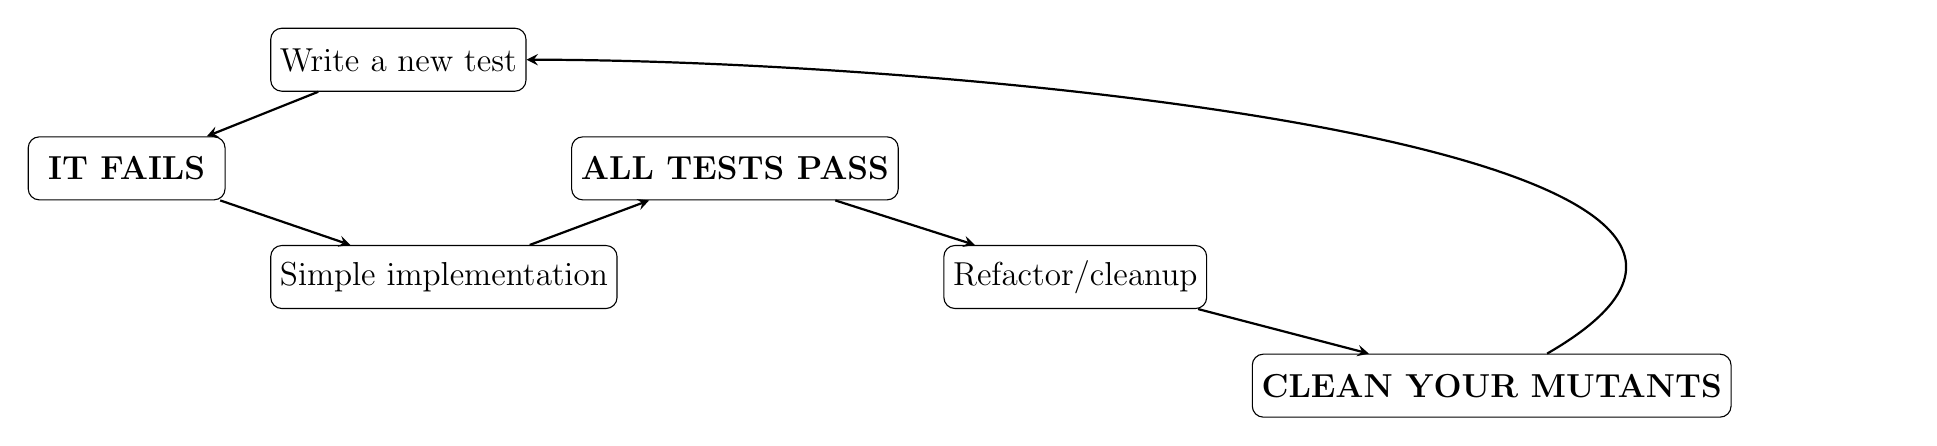
\begin{tikzpicture}[
      font=\large,
      node distance=0.8cm,
      box/.style={rectangle, draw, rounded corners, text centered, minimum width=2.5cm, minimum height=0.8cm},
      arrow/.style={thick,->,>=stealth}
    ]
      \node (write) [box] {Write a new test};
      \node (fail) [box, below left=of write] {{\bf IT FAILS}};
      \node (implement) [box, below right=of fail] {Simple implementation};
      \node (pass) [box, below right=of write] {{\bf ALL TESTS PASS}};
      \node (refactor) [box, below right=of pass] {Refactor/cleanup};
      \node (mutants) [box, below right=of refactor] {{\bf CLEAN YOUR MUTANTS}};

      \draw [arrow] (write) -- (fail);
      \draw [arrow] (fail) -- (implement);
      \draw [arrow] (implement) -- (pass);
      \draw [arrow] (pass) -- (refactor);
      \draw [arrow] (refactor) -- (mutants);      
      \draw [arrow] (mutants) to[out=30,in=0] (write);
    \end{tikzpicture}%
  }
  \caption{Test-Driven Development Loop}
  \label{fig:mdd}
\end{figure}

What does it mean to ``clean your mutants?''  It means that you 1) run
mutation testing \emph{on the file(s) you modified to produce the
  simple implementation} and 2) ensure that every mutant that is not
killed has been inspected and rendered ``clean.''  A killed mutant
(one detected by your tests) is, by definition, clean.

Therefore, one easy way to make a mutant clean is to see that
it indicates a weakness in your testing, and change the tests so it
becomes a killed mutant.  You'll
get to see an inverted version of part of the TDD loop while doing this:  the
modified tests will start failing for the mutated code, once you add power to
the tests, but  they will still pass for the code you wrote for your
actual implementation.

In some cases, you will see that the mutant is semantically equivalent
to the correct code: no reasonable test will ever be able to detect
this change.  It's really just an alternative (perhaps ugly)
implementation.  In this case, you render the mutant clean by
inspecting it.  Once in a while, you might even refactor the
code to remove the annoying mutant (perhaps an even cleaner implementation
wouldn't have this variant?  working at the very small scope of TDD
does seem to give you the freedom to at least consider such
detail-work).  In other cases, you'll have to revisit these mutants
every time you touch these files.  That may be annoying, but it also
means if you were wrong about the semantic equivalence, you get several
chances to notice your mistake.

Calling this new version of TDD ``mutation driven development'' is, frankly,
a bit much.  The new step is intended to be fairly easy to apply, and
to leave the basic structure of TDD unchanged.  My defenses for
the name are
twofold:  first, it sounds nice, and emphasizes the new idea.  Second,
I think there may be a real  argument that ``Test'' in Test Driven Development
is correct but not quite right; the real goal is to drive development
by ``small changes, likely to inflict only small, easily debugged and understood, semantic harm'' ---
which sounds a lot like driving development by mutants.  The tests are
there to make sure the changes really are ``mostly harmless'' as Douglas
Adams might put it; the tests are put in first because you always put
in a safety net \emph{before} you start walking the tightrope.  But
the small scope, easily debugged, carefully constrained, changes are
the real focus, in this vision of TDD, which I think fits with Beck's
original, essentially psychological, argument.  I love tests!  But
tests are a means to an end, in TDD, though also extremely useful in
the end for other reasons.  MDD's purpose is to make sure the
``mutants'' to the code under development aren't simply ``mostly''
harmless but ``almost guaranteed to be entirely harmless.''

\section{Is MDD A Good Idea?}


\begin{figure*}[t]
  {\scriptsize
\begin{verbatim}
mutate src/LedDriver/LedDriver.c --cmd "gcc -c src/util/Utils.c src/LedDriver/LedDriver.c -I include/LedDriver/ -I include/util" --mutantDir LedDriver_mutants/
analyze_mutants src/LedDriver/LedDriver.c "make -f MakefileUnity.mk" --mutantDir LedDriver_mutants/
show_mutants notkilled.txt --sourceDir src/LedDriver/ --mutantDir LedDriver_ mutants | less
\end{verbatim}
    }
  \caption{Commands for mutation testing of LedDriver.c}
  \label{fig:led}
\end{figure*}

I think every developer serious about avoiding bugs should be running
mutation analysis on code as they develop and test it!  So in that
sense, I axiomatically think adding this to TDD would be great, if
you're going to do TDD; you should do this in any case, for code where
you want to make sure you have good tests.

Not everyone is going to be so inherently favorable to mutants,
though, and as I see it the success or failure of the idea really
rests on two empirical claims:

\begin{enumerate}
  \item TDD ensures high enough code coverage and good enough basic
    checking of functionality that looking at unkilled mutants is not
    a major burden on developers.
    \item TDD does not ensure such high quality tests that mutants
      never expose a weakness in testing.
    \end{enumerate}

    As I said above, validating these assumptions empirically is not
    something I've set out to do.  However, I don't want to leave you,
    the reader, without any evidence that this pair of hypotheses
    \emph{might well} be true.  Before I wrote this paper, I decided
    to take two examples of TDD-in-action and check if my claims
    held.  Two is a tiny sample size, and I didn't randomly select
    examples, so this has \emph{no scientific validity}.  However, the
    results convinced me it was worth writing this paper.

    I decided the best way to see if ``good'' TDD might benefit was to
    look at examples of people showing how TDD works.  If TDD-produced
    code by people \emph{showing off the process} had too many
    unkilled mutants for practical application, then MDD is probably
    overly burdensome (and, frankly, I wonder if TDD really works very
    well at the job of producing decent tests); if ``exemplary'' TDD
    on the other hand lacked interesting unkilled mutants, MDD is
    possibly useless, because the benefits will be limited.  You'll
    have to clean many mutants before you find any that actually
    demonstrate weak testing.

    I first looked for a blog post showing TDD in action for Python.
    The first one that came up in search results looked promising:
    \url{https://pytest-with-eric.com/tdd/pytest-tdd/}.  I took the
    code, cleaned it up (the blog post has some code with typos) and
    followed along with the TDD example, applying mutation testing at
    each stopping point (just before a new test was added).

    The versions I produced are available in github
    (\url{https://github.com/agroce/mdd/tree/main/pytestwitheric}).  I
    used my own mutation testing tool, the Universal
    Mutator~\cite{SyntaxUM}
    (\url{https://github.com/agroce/universalmutator}, to generate
    mutants.

    If you want to follow along at home, the easiest way to do so is
    to download the docker image in which I carried out my
    ``experiments.''

 \begin{code}
 docker pull agroce/mdd
 docker run -it agroce/mdd
 cd ~/mdd/pytestwitheric/
 \end{code}

The code is organized into ``versions'' I extracted from the blog
post, numbered {\tt v1} through {\tt v6}.  It's a good idea to look at
the code in each of these directories and match it up to the code from
the blog post before proceeding; this will give you an idea of the
``lay of the land''.
 
    Then, to try out MDD, go into any directory, e.g. {\tt v3}, and type:

 \begin{code}
 cd v3
 mutate string\_manipulator.py
 analyze\_mutants string\_manipulator.py "pytest"
\end{code}

You'll see the universal mutator tool producing a set of valid mutants
of the version of the code, followed by actual mutation testing.  For
the first version, {\tt v1}, there are no mutants.  Clean by the
empty set!  For version {\tt v2}, there are two mutants, and both are
detected.  For version {\tt v3}, there are six mutants, again all
detected. For {\tt v4} the number of mutants grows to nine, still all
detected.  With {\tt v5} we get fifteen mutants (for about ten lines
of code), still all detected.  So far, we've gained nothing, but we've
also done no real additional work (running the mutants takes less than 4
seconds, inspecting the result in case of 100\% killed mutants is trivial).

And then with {\tt v6}, we see that three mutants are not killed. Our
score drops to 87.5\% killed mutants.  The three surviving mutants are
all similar, so we can examine only the first one:

{\scriptsize
\begin{code}
show\_mutants notkilled.txt 

MUTANT \#1:
string\_manipulator.mutant.18.py: ./string\_manipulator.py:13
*** Original
--- Mutant
***************
*** 10,15 ****
          if not my\_string:  
              return "String is empty"  
          if not isinstance(my\_string, str):  
!             return "Invalid input"  
          new\_string = my\_string.replace(pattern, "")  
          return new\_string
--- 10,15 ----
          if not my\_string:  
              return "String is empty"  
          if not isinstance(my\_string, str):  
!             return ""  
          new\_string = my\_string.replace(pattern, "")  
          return new\_string
        \end{code}
      }

 We wrote code for the case where an input to our function isn't a
 string, but we didn't write a test checking that this does what we
 expect when we pass a non-string.  The test is easy to add:

 \begin{code}
def test\_remove\_pattern\_type\_int():
     sm = StringManipulator()
     res = sm.remove\_pattern(3, "Eric")
     assert res == "Invalid input"
   \end{code}

   Once we add it (in my version {\tt v6.FIX}), we're back to 100\%
   killed mutants.  Great!

   This is simply a toy example from a blog post; what about more
   ``respectable'' demonstration of TDD?

   Taking the first example from the excellent Grenning
   book~\cite{grenning}, we can look at the final version of the code
   and tests for a simple LED driver.

\begin{code}
cd ~/tddec-code/code
\end{code}

Producing mutants and analyzing them is now more complex
(Figure~\ref{fig:led}).  We kill almost 90\% of the 98 generated
mutants.  But, importantly, we don't kill them all.  The few mutants
remaining show that, despite the tests including a number of checks
for correct behavior when LED numbers are out of bounds, these tests
\emph{don't catch all the possible cases}:  the ten mutants not killed
show that some bounds checks are indeed tested, but others are not;
changing the {\tt enum} to incorrectly label the LEDs also can get
past the tests (wrong numbering is a problem Grenning specifically
calls out).  The tests \emph{mostly} catch these problems, but they
don't catch \emph{all} of them.  And as far as I can tell, the mutants
not killed all indicate these exact problems.  Is looking at ten
mutants a huge burden on a developer?  I think not, at least in this
case.  As soon as you see one mutant showing bound checks aren't being
fully probed, you probably will quit looking at mutants and proceed to
strengthen the tests to cover bounds tests more effectively.  After
that minor effort, the likely outcome (for this code) is 100\%
mutation score.

Perhaps these examples aren't typical, but I think they are
sufficiently compelling to make a case for trying out MDD, if you
currently practice TDD.  Let me know if it works for you (or if you
are an eager graduate student dying to turn this sketchy idea into a ``real'' paper)!

\section{The Mighty River: A Digression}

This is an essay (thus a jackdaw, magpie, raven~\cite{doyleessay}), not a research paper, so we can turn our minds aside
for a moment.  The real reason I couldn't let MDD simply fall into the
junkyard of never-pursued research ideas without making some effort to put it
out in the world for serious consideration is that it fits into a
larger vision I have of software engineering, or in particular, of
``coding'' --- the kind of vision you
can only talk very very briefly about in a research paper in a short lyrical passage in the
introduction that still annoys at least one ICSE reviewer.

Mark Twain's \emph{Life on the Mississippi} is one of the best books
ever written.  And one thing it makes you \emph{see}, that you may
never have seen before, if you haven't read it, is how a river pilot
had to know the river.  Much of the first part of the book is taken up
by the tale of young Clemens/Twain learning to be a river pilot; at
first the task of knowing the ever-changing, infinitely complex, night
and day and many-season Mississippi simply seems impossible.  And
every time young Twain thinks, cockily, that he \emph{has} done this
impossible thing, the irascible expert pilot Bixby tells him something
else insanely difficult he has to know:

\begin{quote}
``Then I've got to work and learn just as much more river as I already
know.''

``Just about twice as much more, as near as you can come at it.''

``Well, one lives to find out.  I think I was a fool when I went into
this business.''

``Yes, that is true.  And you are yet.  But you'll not be when you've
learned it.''

``Ah, I never can learn it.''

``I will see that you DO.''
\end{quote}

This was written when the river had no lights or bouys, and we may
think that it is fun to learn, but not very relevant to  our work, not
being river pilots, and the world having advanced to add lights and
buoys by the time Twain wrote, much less by our far future day.  But
what Twain is really talking about is how well we have to know code,
if we want it to be correct.  You have to know your code like a pilot
knows the river; and the river is ever-changing and our code, itself,
and the context it lives in, is ever-changing.

\begin{figure}
  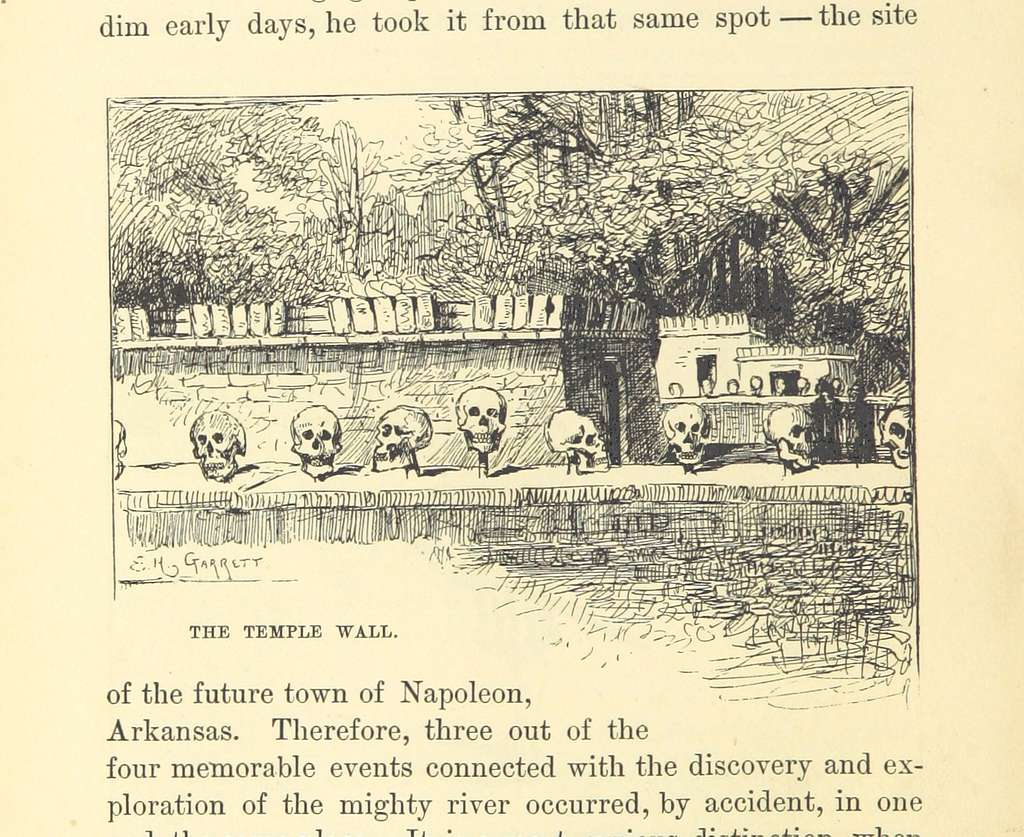
\includegraphics[width=\columnwidth]{twain.jpg}
  \caption{Illustration from 1883 J. R. Osgood and co. edition of Mark
  Twain's \emph{Life on the Mississippi}, source \url{https://renopenrose.getarchive.net/media/44-of-life-on-the-mississippi-by-mark-twain-samuel-l-clemens-with-more-than-bef073}}
  \label{fig:twain}
  \end{figure}

I think the change in point of view from code coverage (handled by
TDD) to mutation (added by MDD) is like one of those sudden
enlargements of the notion of the river a pilot has to carry about all
inside poor Mark Twain's young head:  you thought you knew the river
when you knew this (every bend and turn, every plantation and how it
all looks at night when you can't really see it), but in fact you have
to know \emph{this} as well (how to read the river's ``dynamics'' from
the height of every single bank you see).  Figure \ref{fig:twain}
shows what happens to those who do not know the river well enough, or
at least to the users of their software.

Coverage (TDD's forte; you not only have good coverage, but you have
in your head the map of how you got that coverage, painstaking loop of
failure, then new code, then pass, and once more failure to code to pass) is the river's basic
shape; mutation (MDD's addition) shows you part of the changing shape
of the river as it runs as well; mutation is a \emph{text-driven} form
of insight into the ``shape'' of the dynamic state space, not just the
``textual space'' of the code.  The vision of TDD, as I see it, is to
give a developer the confidence of an expert river pilot, not only the
ability to avoid destroying a boat, but the bold power to still
maintain speed while maintaining safety.  The ideal of the process of
TDD is to embody the teacher Bixby as a process to be followed; the
promise of MDD is to make Bixby as demanding as the real Bixby Twain
wrote about, and to make TDD form real river pilots.  Does it work?  I
don't know; someone will have to try it on the actual river.

\section{A Bigger Picture}

If (it's a big if) MDD is a useful idea, I think it's a minor example
of where we get many nice ideas:  cross-overs.  I don't ``do'' TDD and
I think people who are interested in TDD in the research world are
mostly (I would guess, I don't read much TDD literature) ``process''
people.  I think ``process'' people who care about TDD probably think
a lot about testing, but don't think very deeply about code coverage
metrics (beyond the basic ``let's see what ran'') or the ``oracle
problem''~\cite{staats2011programs,oracleMcMinn} because these ideas are mostly siloed into the ``tools and
automated test generation'' part of the larger SE world.  I happened
to start thinking about TDD because while I usually taught CS 362, the
``testing and debugging'' class at Oregon State, one semester I was
asked to do CS 361, the ``design and process'' class.  TDD seemed like
the most ``hardcore testing people'' thing to learn for that class,
and sounded interesting, even if I had no particular interest in
agile/XP/any of that ``stuff.''  I didn't know at the time Grenning
had a very good book applying all this to the embedded world, which I
\emph{did} care about.

Because I'm always thinking about mutation and mutants, I wondered if
TDD gave rise to really great mutation scores, since it not only
encourages coverage, but pushes for code to be written in tandem with
good functionality probes.  That mildly ``across disciplines''
thought, following an inspection of the mutation scores for 80+
students over their TDD versions of KWIC,
gave rise to the notion of MDD.  But TDD is in the ``process'' and
``people'' and ``agile'' boxes, not in any of my boxes (``test
generation'', ``fuzzing'', ``test suite evaluation measures''), so I
put it aside.  And had I not read Jackson's book, likely MDD's only
existence would be as a thing I occasionally mentioned to people I knew.

In her fascinating new history of the Renaissance~\cite{palmer}, Ada
Palmer notes that ``major discoveries often come from someone studying
a different topic asking new questions'' --- in her epistemological
(and thus extremely pleasing to a ``testing guy'') version of history,
this is a key to understanding:  you need to look at a ``thing'' from so many
viewpoints that the connections between viewpoints become clear.  This
can even expose ``new''
facts (this event happened less than a week before
this other similar event, and was done by the same guy, that means
they are really \emph{part of the same story}) even where technically,
everyone has ``known'' about the new facts forever, it's just that
nobody ever actually \emph{looked} at those facts.  I think Jackson's
point about research that is just hard to evaluate, or where the mashup of fields
involved may make a Busy Professional Professor Researcher reluctant
to do anything with a basic partly-out-of-my-field idea, comes into play here:  if the standards are
always to be rooted in rigorous experimental work (RQs 1-6 evaluated
using the right statistics and a compelling base of data from human
subjects or mined from software repositories, pleasing to everyone on
the ICSE PC!), we're going to miss those connections sometimes.
That, in my opinion, even if MDD in particular isn't a very useful
idea, is a shame.  Even if I'm not, \emph{the rest of you} are probably having lots of
slightly out-of-band good ideas all the time, and I fear you're
burying them because they don't quite fit the model of the way we do
``research'' now.

\bibliographystyle{ACM-Reference-Format}
\bibliography{bibliography}



\end{document}